%%% template.tex
%%%
%%% This LaTeX source document can be used as the basis for your technical
%%% paper or abstract. Intentionally stripped of annotation, the parameters
%%% and commands should be adjusted for your particular paper - title, 
%%% author, article DOI, etc.
%%% The accompanying ``template.annotated.tex'' provides copious annotation
%%% for the commands and parameters found in the source document. (The code
%%% is identical in ``template.tex'' and ``template.annotated.tex.'')

\documentclass[annual]{acmsiggraph}
\usepackage{subfigure}
\TOGonlineid{45678}
\TOGvolume{0}
\TOGnumber{0}
\TOGarticleDOI{1111111.2222222}
\TOGprojectURL{}
\TOGvideoURL{}
\TOGdataURL{}
\TOGcodeURL{}

\title{3D face hallucination from a single RGBD image}

\author{Robert A. Smith\thanks{e-mail:rsmith@gmail.com}\\Smith Research}
\pdfauthor{Robert A. Smith}

\keywords{radiosity, global illumination, constant time}

\begin{document}

%% \teaser{
%%   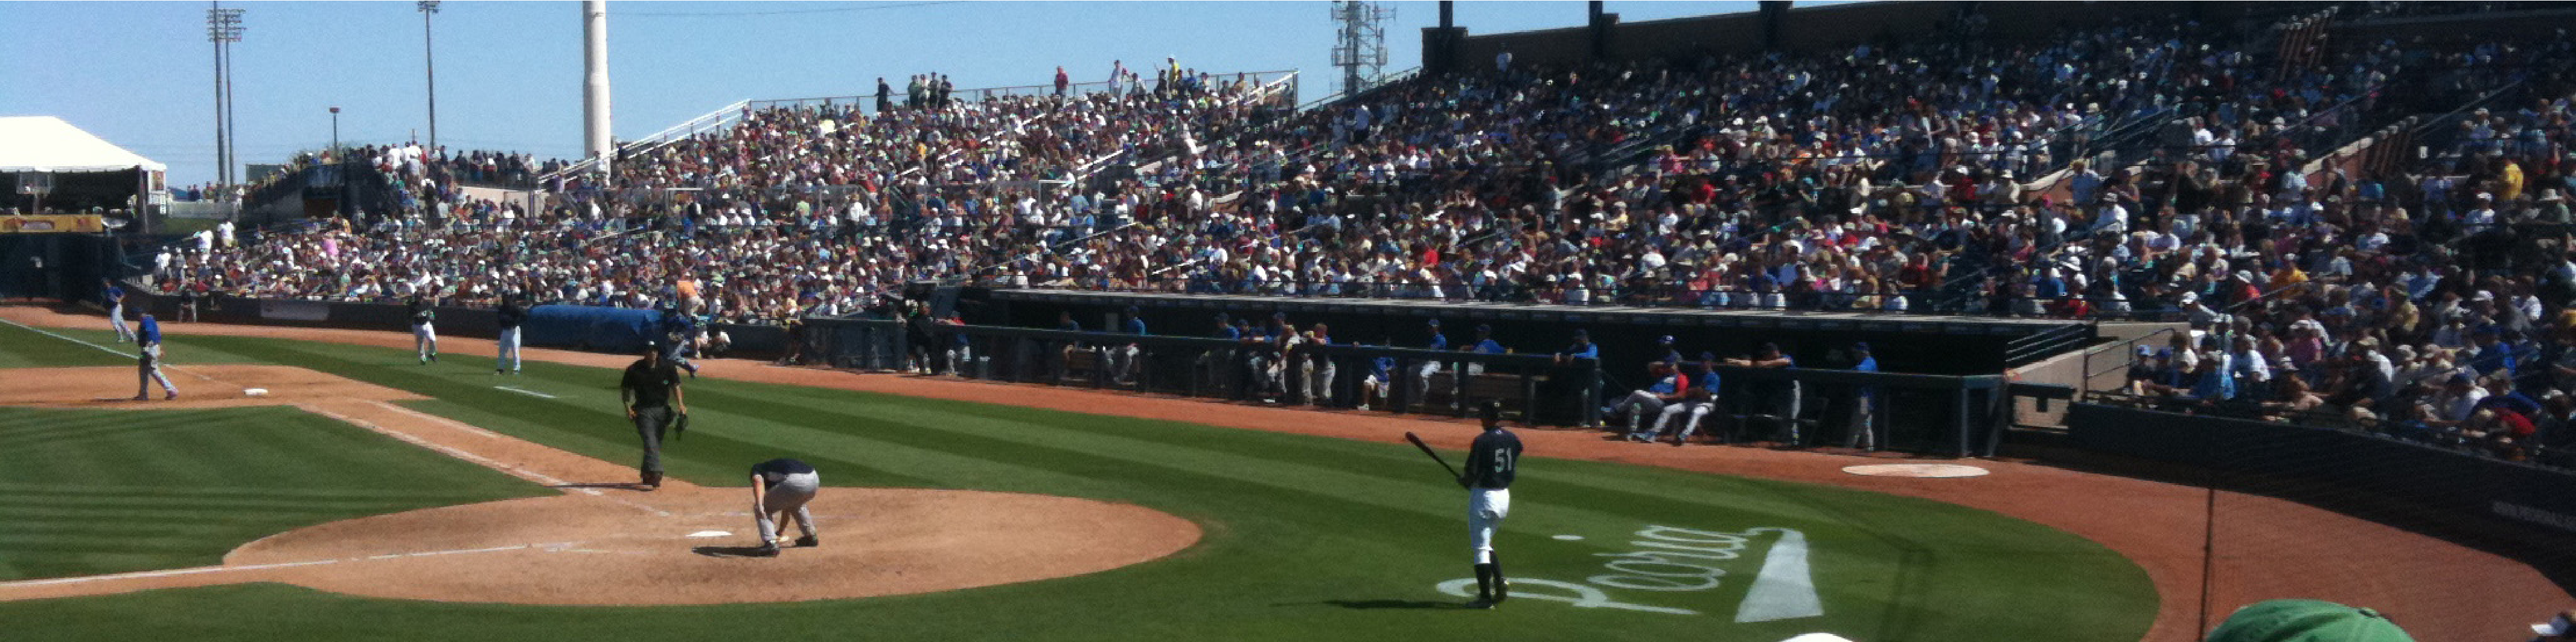
\includegraphics[height=1.5in]{images/sampleteaser}
%%   \caption{Spring Training 2009, Peoria, AZ.}
%% }

\maketitle

\begin{abstract}

Duis autem vel eum iriure dolor in hendrerit in vulputate velit esse
molestie consequat, vel illum dolore eu feugiat nulla facilisis at 
vero eros et accumsan et iusto odio dignissim qui blandit praesent
luptatum zzril delenit augue duis dolore te feugait nulla
facilisi. Lorem ipsum dolor sit amet, consectetuer adipiscing elit,
sed diam nonummy nibh euismod tincidunt ut laoreet dolore magna
aliquam erat volutpat.

Citations can be done this way~\cite{Jobs95} or this more concise 
way~\shortcite{Jobs95}, depending upon the application.

Ut wisi enim ad minim veniam, quis nostrud exerci tation ullamcorper
suscipit lobortis nisl ut aliquip ex ea commodo consequat. Duis autem
vel eum iriure dolor in hendrerit~\cite{Pellacini:2005:LAH}
in vulputate velit esse molestie~\cite{notes2002} 
consequat, vel illum dolore eu feugiat nulla facilisis at vero eros et
accumsan et iusto odio dignissim qui blandit praesent luptatum zzril
delenit augue duis dolore te feugait nulla facilisi.~\cite{Park:2006:DSI}

\end{abstract}

\begin{CRcatlist}
  \CRcat{I.3.3}{Computer Graphics}{Three-Dimensional Graphics and Realism}{Display Algorithms}
  \CRcat{I.3.7}{Computer Graphics}{Three-Dimensional Graphics and Realism}{Radiosity};
\end{CRcatlist}

\keywordlist

\TOGlinkslist

\copyrightspace

\section{Introduction}



\section{Related Work}




\section{Data Format}

Our dataset consists of 1204 Caucasion individuals ranging from 3 to 40 with males and females. The high-resolution 3D facial meshes are obtained from a 3dMD digital stereophotogrammetry imaging system(Atlanta,GA). These systems are outfitted with multiple CCD cameras mounted at fixed angles and distances, to capture overlapping views of the faces and heads. Each of the 3D heads comprises of 30-40,000 points and subjects are all in neutral expressions. Subjects were required to wear caps to get rid of the hairs that obscure their faces. Before the experiment, the meshes were cleaned and pose-normalized using a method described in ~\cite{wilamowska2009classification}. 22 anatomical facial landmarks were labeled manually on each surface by a single trained medical expert as shown in Fig.\ref{dataset}. With a generic face mesh and 22 landmarks, deformable registration is applied to all the meshes so that they all have dense correspondences to each other~\cite{allen}. We manually placed 83 landmarks on the generic face mesh $G$ and transfer them to all the meshes accordingly.  These 83 landmarks are very crucial in determing different facial component regions as well as helping to warp the dataset towards Kinect input face.Also, we divide the generic face into 5 facial components, namely Eyes, Nose, Mouth, LeftCheek and RightCheek as shown in Fig. \ref{pipeline}. 

\begin{figure}[ht]
  \centering
  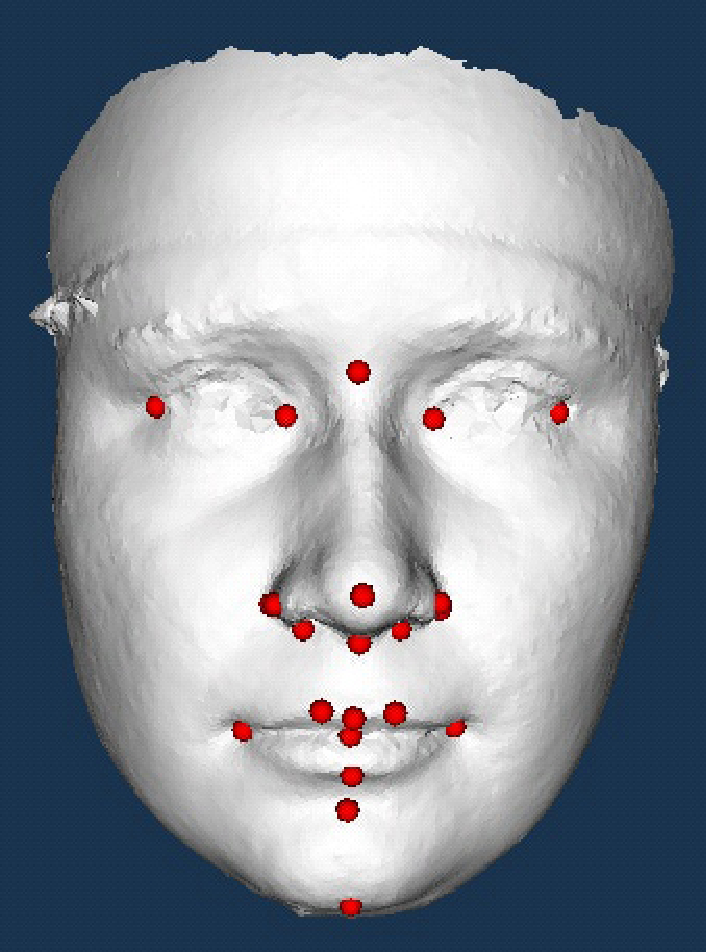
\includegraphics[width=1.5in]{images/dataformat}
  \caption{High resolution 3dMD facial mesh with 22 anatomical landmarks}\label{dataset}
\end{figure}


\section{Overview}
The pipeline of our method is show in Fig. \ref{pipeline}. Given a single RGBD frame of a person's frontal face, we first use the toolkit FacePlusPlus ~\cite{face++} to generate 83 facial landmarks on the color image. Then, we transfer the 2D landmarks $M$ to 3D points $P$ according to the depth image using the caliberated camera projection matrix. The face region is cropped out with the help of the $P$ and the 3D point cloud is connected to form a mesh $O$. The Kinect raw input is smoothed using curvature flow to reduce noise in the original mesh, denoted as $S$. Since landmarks $P$ on face contour can be inaccurate if just inferred the frontal view, we pick 15 anatomical landmarks $P_{15}$ to align the input to our generic face model $G$. With the help of the 15 landmarks, we deform our generic face model to $S$ to generate a dense correspondence. In case that the exact same face for $S$ doesn't exist in our dataset, we warp all the face meshes in our dataset towards $S$ using the 83 landmarks $P$. We retrieve for the most similar facial component for each of the 5 facial parts in $S$ among the deformed dataset. After we get the most similar high-resolution facial component, we transfer the vertex normals from the HR mesh to the Kinect smoothed mesh $S$ and use the normal-correct-positon method to generate our final HR 3D mesh. Note that here, we just use the corresponding information to find masks for each facial components and we don't want to use the deformed generic shape to represent the input shape. Our further steps of similarity comparison and combining normals with points are still performed in the Kinect input space. 

\begin{figure*}[htb]
  \centering
  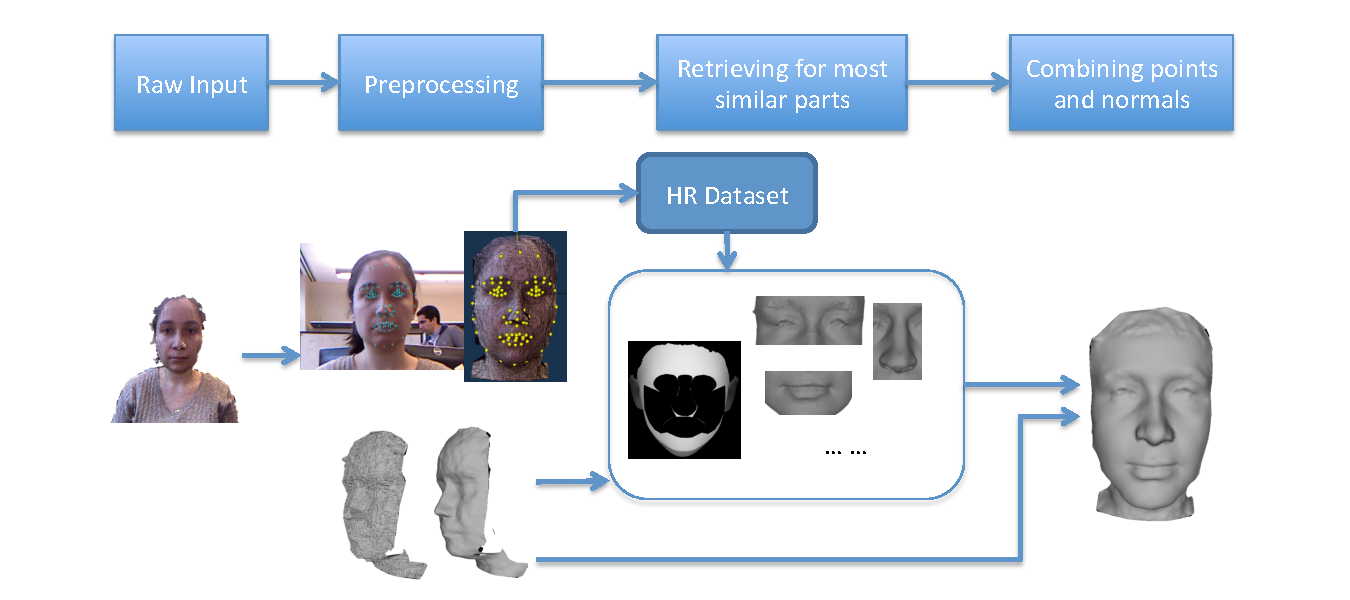
\includegraphics[width=8in]{images/pipeline}
  \caption{Overview of the pipeline}\label{pipeline}
\end{figure*}

\section{Preprocessing of Kinect raw input}
Our subject is required to stay right in front of Kinect and keep a neutral expression for a few seconds with pose nearly normalized. Then a single RGBD frame is collected and sent to our reconstruction system.

The purpose of preprocessing Kinect raw input is to a) align it to our dataset b) generate facial component masks c) initialize it for HR facial components retrieval.

\textbf{Landmark Labeling} Since the Kinect raw input O is noisy and consists of hole regions, it is not easy to generate 3D landmarks directly from 3D shapes.  We then apply 2D face alignement method to the color map to get 2D landmarks $M$ and transfer them to 3D space. Any face alignment method can be used in this step, here we use FacePlusplus~\cite{face++} to generate 2D landmarks as well as extracting face region out. These landmarks are transferred into 3D space using caliberated camera projecton matrix. These 83 landmarks include 19 contour points and 64 facial points. Since facial contour points depend on the face pose and can not always be correspondent on 3D meshes, we just use 15 anatomical 3D landmarks  $P_{15}$ for pose alignment as shown in Fig. \ref{landmarks}.

\begin{figure}[ht]
  \centering
\subfigure[]{
  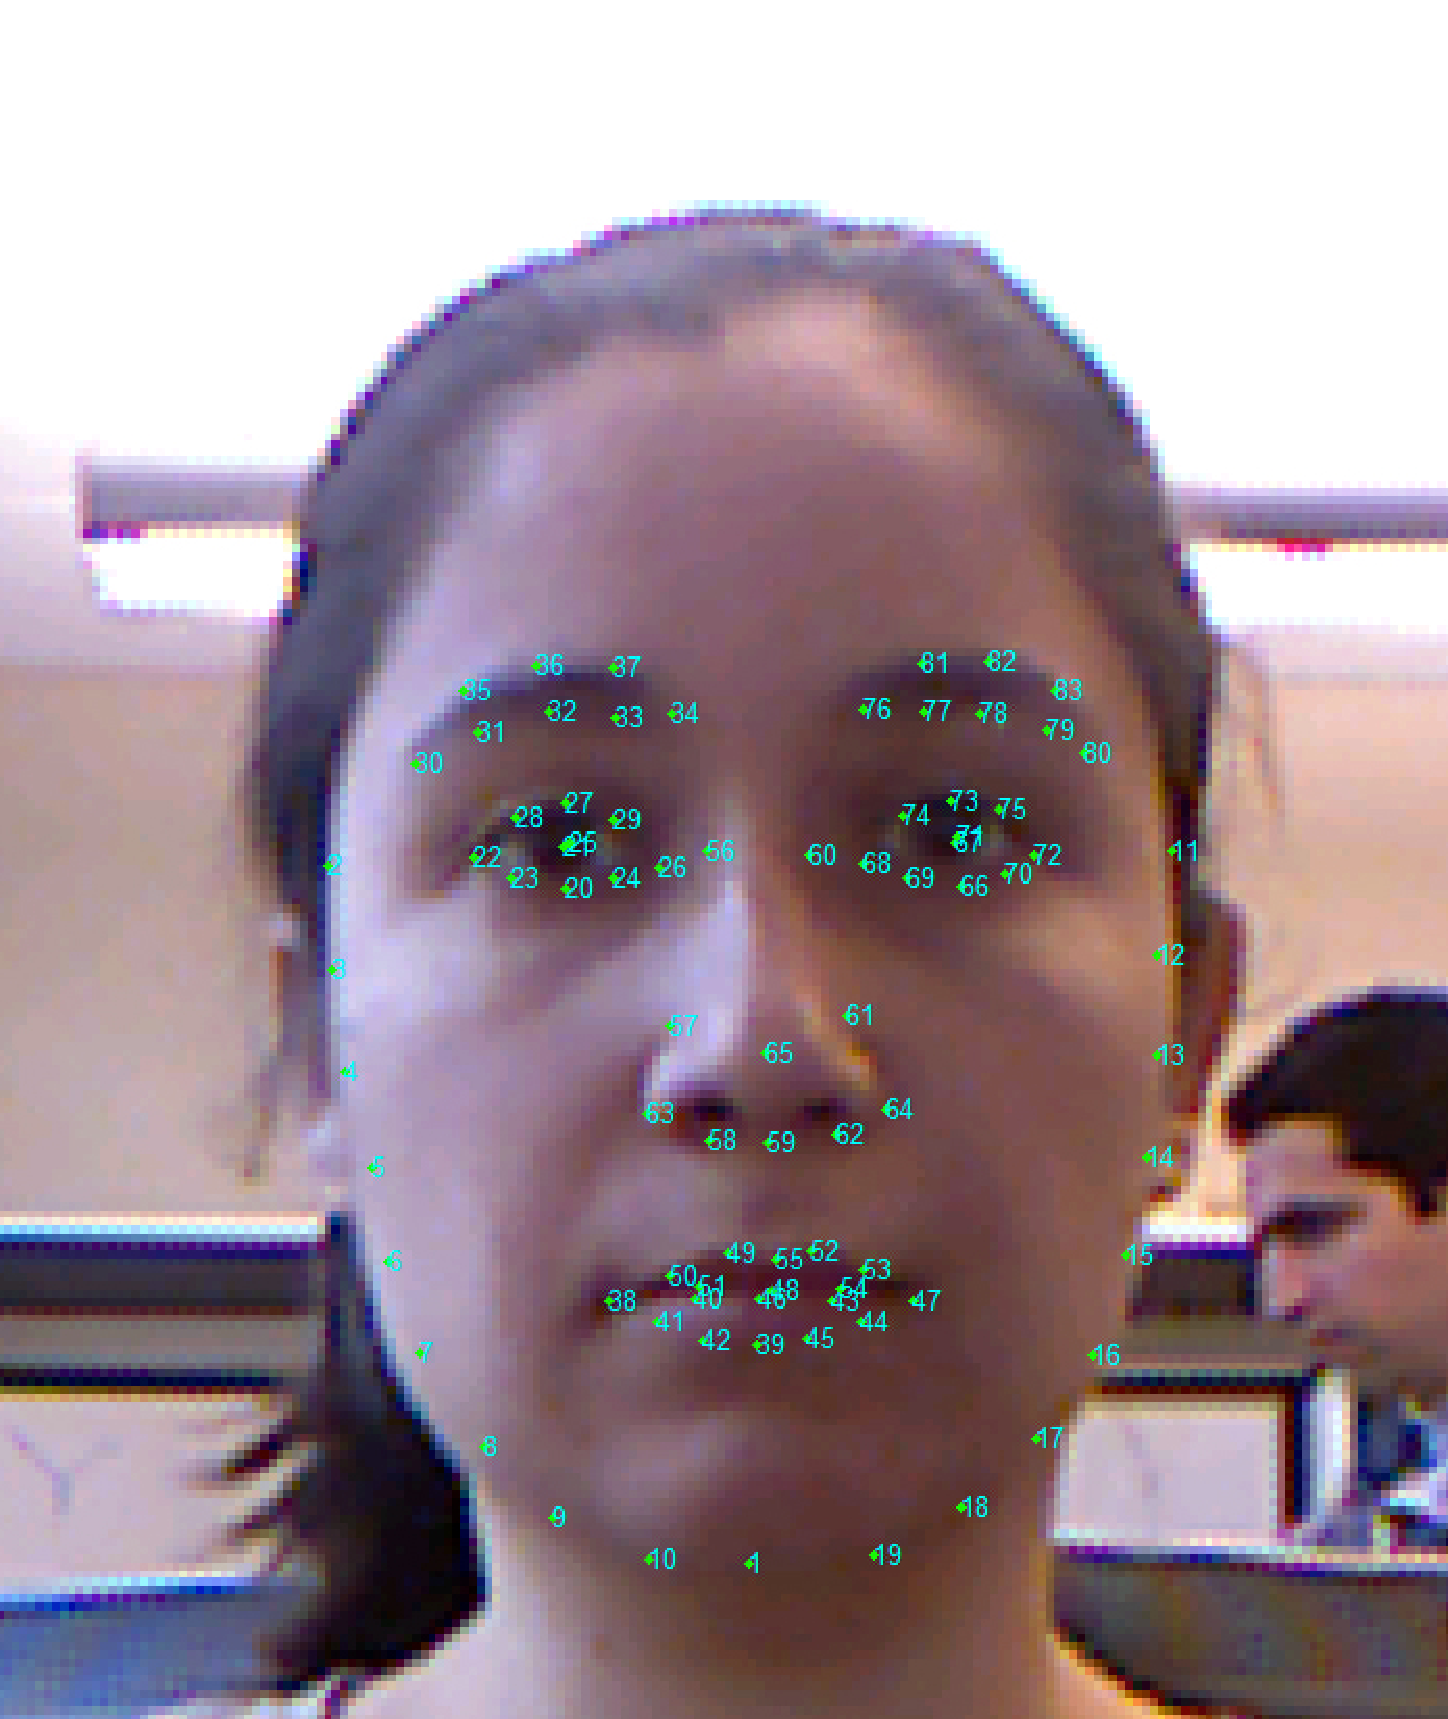
\includegraphics[width=1in]{images/83points}}
\subfigure[]{
  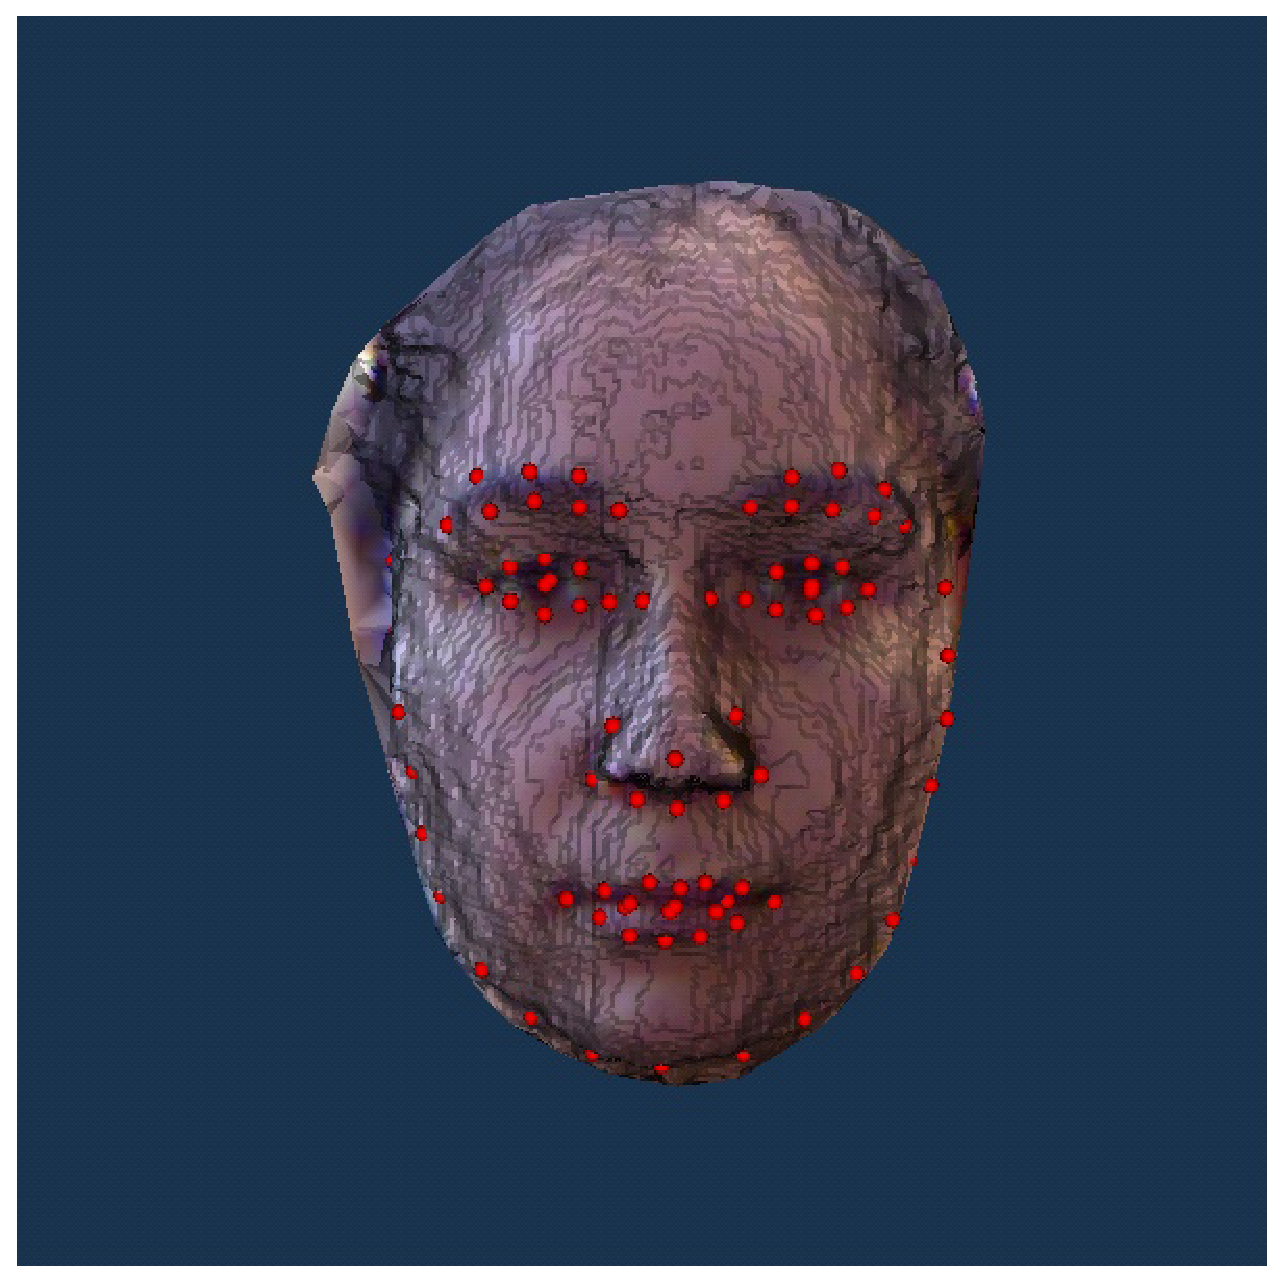
\includegraphics[width=1in]{images/alignedface} }
\subfigure[]{
 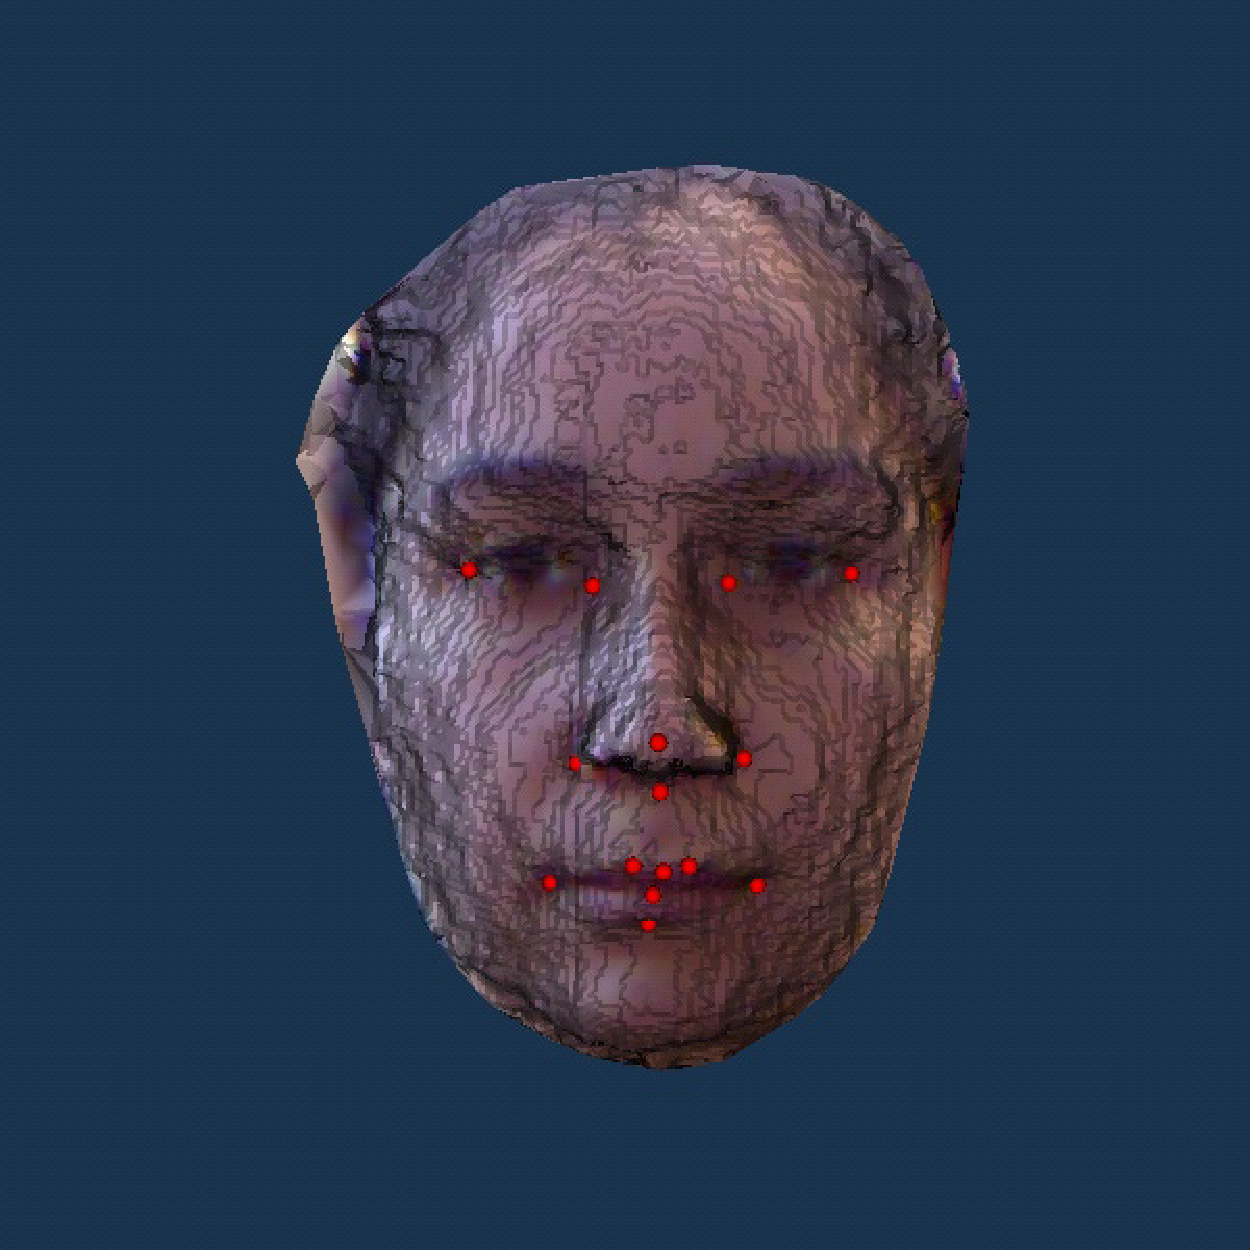
\includegraphics[width=1in]{images/15landmarks}}
  \caption{Landmarks Labeling.(a) shows the 83 landmarks detected on 2D color image. (b) shows the transferred landmarks on 3D mesh $O$. (c) shows the 15 anatomical landmarks used for face alignment and deformable registration}\label{landmarks}
\end{figure}


\textbf{Mesh Smooth} Because of the inaccuracy of Kinect depth sensor, the reconstructed mesh $O$ is very noise and it is hard to infer too much human feature from that. To retrieve for similar high resolution facial components, a mesh smooth method is performed on Kinect raw input $O$. Rather than do the filtering on 2D depth map, we apply curvature flow smooth method directly on $O$. The curvature flow smooth method is good at keeping low frequency shape meanwhile smoothing out high frequency noises. Note the Figure in Fig. \ref{smoothed}. After the curvature flow smooth, we can see the general shape of the face more clearly.

\begin{figure}[ht]
\centering
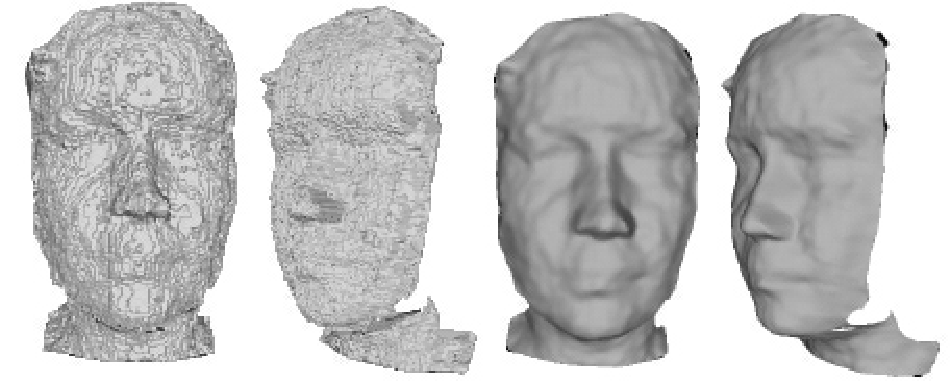
\includegraphics[width=3in]{images/smoothed}
\caption{Raw Kinect input mesh and smoothed mesh(frontal view and side view)}\label{smoothed}
\end{figure}

\textbf{3D Mesh Alignment} Although the RGBD image is taken from the frontal view, there are still some yaw or roll rotations in the subject's head pose. Given $P_{15}$ and the corresponding landmarks on $G$, Procrustes Analysis is used to align the original mesh to our dataset. 
To get dense correspondence from $S$ to $G$, we use deformable registration method proposed in ~\cite{allen}. The energy to be minized for dense matching is defined as
\begin{equation}
E={\alpha}E_d+{\beta}E_s+{\gamma}E_m
\end{equation}
where $E_d$ represents the data error, $E_s$ represents the smoothness error and $E_m$ is the landmarks error between our 15 3D landmarks $P_{15}$ on $S$ to the landmarks on $G$. The process is iterative. In early stages, the landmark error $E_m$ contributes more to the global optimization. As the process moves on, the data error $E_d$ dominates the optimization.\\
Once the deformable registration is done, we can obtain the masks for each facial component on $S$ transferred from $G$.

\textbf{Warpped HR Dataset} Although our dataset consists of over 1,000 3D face meshes, it is not necessary that any of our Kinect input low resolution head can find the exact similar facial components within our dataset. To be more general, all 3D face meshes in our dataset are warpped towards $S$ according to the 83 landmarks. Since the landmarks on $S$ can be quite inaccurate in $z$-direction, we just warp our dataset using $x,y$-coordinate of the landmarks. Here, RBF method is used to warp all face meshes in the high resolution dataset.

\section{Retrieval for the most similar HR facial components}
The distance between a query facial component and all the corresponding facial components in our dataset can be defined as

\begin{equation}
E=E_p+{\alpha}E_{angle}
\end{equation}
where $E_p$ reprenset the distance of pseudo-landmarks and $E_angle$ is the distance between two Elevation-Azimuth Histograms.

\textbf{Pseudolandmarks} are a set of 3D landmarks that cover the entile facial part as shown in Fig.\ref{pseudolandmarks}. Pseudo-landmarks can be viewed as a downsampling result of face shape, which cover the whole face region and represent the general shape of one's face.
\begin{figure}[ht]
  \centering
  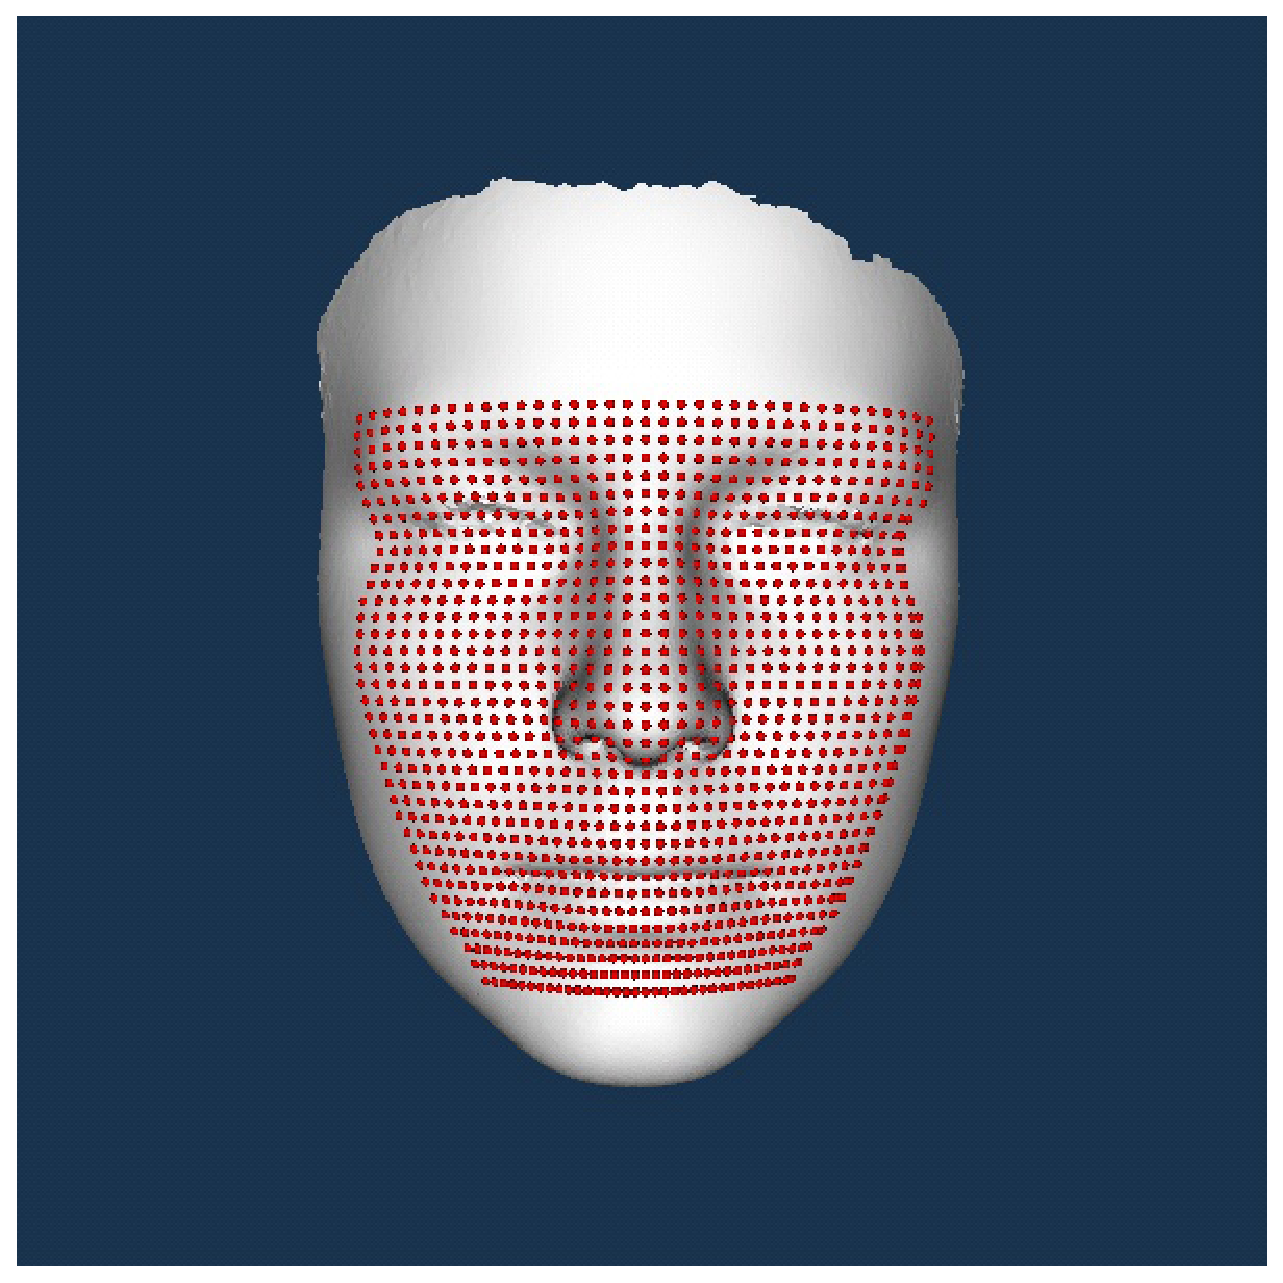
\includegraphics[width=1.5in]{images/pseudolandmarks}
  \caption{Pseudolandmarks on our generic shape $G$}\label{pseudolandmarks}
\end{figure}

We calculate pseudo-landmarks for smoothed Kinect mesh $S$ using the method proposed in XXX. They proposed a very simple, but effective method that computes pseudo-landmarks by cutting through each 3D head mesh with a set of horizontal planes and extracting a set of points from each plane. The method starts with a 3D head mesh pose-normalized to face front. It computes two anatomical landmarks, the sellion and chin tip fully automatically and constructs horizontal planes through these points. With these two planes as base planes, it constructs $m$ parallel planes through the head and from each of them samples a set of $n$ points. In our retrieval, we set $m$ as 33, $n$ as 35. Then, 35$\times$35 pseudo-landmarks are computed to represent a face, we will present that such resolution is enough for representing face shapes in the following sections.
Pseudo-landmarks are computed on the whole face region for all the warpped HR 3D mesh and smoothed input mesh $S$. The similarity score for each warpped HR mesh compared to query mesh $S$ is 

\begin{equation}
E_p=\sum_{i=1}^{1225}{||L_i-Lq_i||^2}
\end{equation}
where $L_{i}=(x_i,y_i,z_i)$ represents a xyz-coordinate of a pseudo-landmark on a HR mesh and $Lq_{i}$ is the coordinate for $S$.

\textbf{2D Elevation-Azimuth Histogram} Given the normal vector $n(n_x,n_y,n_z)$ at a 3D point, the azimuth angle $\theta$ is defined as the angle between the positive $x$-axis and the projection of $n$ to the $xy$ plane, $n'$. The elevation angle $\phi$ is the angle between $x$-axis and $n$.

\begin{equation}
\theta=arctan(\frac{n_z}{n_x}) ,         \phi=arctan(\frac{n_y}{\sqrt{({n_x}^2+{n_z}^2)}})
\end{equation}

Here $\theta{\in}[-\pi,\pi]$, $\phi{\in}[-\frac{\pi}{2},\frac{\pi}{2}]$.

With azimuth and elevation angles, any unit vector in 3D space can be defined. With a 2D histogram, the orientation variaty of a surface can be represented according to the normal direction of all its vertices. On relatively flat regions of a head, all point normal vector point in the same direction, which will cause a strong signal in some bins of the 2D histogram as show in Fig. \ref{AEhist}. In our dataset, a 32$\times$32 histogram is used for each facial component. So each facial component can be represented by a 32$\times$32 matrix M. Then the angle distance $E_{angle}$ can be defined as 

\begin{equation}
E_{angle}=||M-M_q||
\end{equation}

\begin{figure}[ht]
  \centering
  
\includegraphics[width=3in]{images/AEhist}
  \caption{Elevation-Azimuth Histogram of a 3D face}\label{AEhist}
\end{figure}

Pseudo-landmarks and 2D Elevation-Azimuth histogram can be computed for the whole face region as well as for separate facial components. Rember that we divide the whole face region into 5 components: nose, eyes, mouth, left cheek and right cheek. We retrieve for the most similar part for them separately. For nose region, where the depth of each point varies a lot, we choose a small $\alpha$ value. For eyes and mouth regions, where normal angles vary a lot, we enlarge $\alpha$ value to let the normal angle feature contributes more.
 
\section{Combining HR details with Kinect input}
Once we get the most similar HR facial components for each facial part, we can use the normal information from the HR parts to improve our smoothed mesh $S$. 

\section{Experiment and results}



\section{Conclusion}


\section*{Acknowledgements}

To Robert, for all the bagels.

\bibliographystyle{acmsiggraph}
\bibliography{template}
\end{document}
